\documentclass{article}
%\usepackage[latin1]{inputenc}
\usepackage{graphicx,amssymb,amsmath,amsbsy,MnSymbol} % extensions pour maths avancées
\usepackage{graphicx}           % extensions pour figures
\usepackage[T1]{fontenc}        % pour les charactères accentués 
\usepackage[utf8]{inputenc} 

\usepackage{stmaryrd} % Pour les crochets d'ensemble d'entier
\usepackage{float}  % Pour placer les images là ou JE veux.

\DeclareMathOperator{\tr}{tr}
\DeclareMathOperator{\argmax}{argmax}


\setlength{\parindent}{0.0in}
\setlength{\parskip}{0.3in}
\setlength{\topmargin}{-0.4in}
\setlength{\topskip}{1in}    % between header and text
\setlength{\textheight}{8in} % height of main text
\setlength{\textwidth}{4.5in}    % width of text
\setlength{\oddsidemargin}{1in} % odd page left margin
\setlength{\evensidemargin}{1in} % even page left margin
%
%% Quelques raccourcis clavier :
\def\slantfrac#1#2{\kern.1em^{#1}\kern-.3em/\kern-.1em_{#2}}
\def\b#1{\mathbf{#1}}
\def\bs#1{\boldsymbol{#1}}
\def\m#1{\mathrm{#1}}
%
\newcommand{\greeksym}[1]{{\usefont{U}{psy}{m}{n}#1}}
\newcommand{\inc}{\mbox{\small\greeksym{d}\hskip 0.05ex}}%
\pagenumbering{arabic}
\date{\today}
\title{DM2: Modèles Graphiques}
\author{Barbara Gris \& Nelle Varoquaux}
\begin{document}
\maketitle
\tableofcontents{}
\vfill \eject

\section{Distributions factorisables dans un graphe}
\subsection{Question a}

Soit $G = (V, E)$ et soit $i \rightarrow j$ une arête couverte, i.e, telle que
$\pi_j = \pi_i \bigcup \{i\}$.
Soit $G'= (V,E)$, avec $E' = (E \setminus \{i \rightarrow j\}) \bigcup \{j \rightarrow i\}$.

Montrons que $\mathcal{L}(G) = \mathcal{L}(G')$


Par définition, on a:
\begin{align}
\mathcal{L}(G) & = & \{ p \mid p(x) = \prod_{k = 1}^{n} p(x_k \mid x_{\pi_k}) \} \\
	       & = & \{ p \mid p(x) = A p(x_i \mid x_{\pi_i}) p(x_j \mid x_{\pi_j} \}
\end{align}

avec $A = \prod_{k \in V \setminus \{i, j\} p[x_k \mid x_{\pi_k}]}$. De même, on a:

\begin{align}
\mathcal{L}(G') & = & \{ p \mid p(x) = \prod_{k = 1}^{n} p(x_k \mid x_{\pi'_k}) \} \\
		& = & \{ p \mid p(x) = A p(x_i \mid x_{\pi'_i}) p(x_j \mid x_{\pi'_j} \}
\end{align}

De plus,

$$\pi_j = \pi_i \bigcup \{ i \}$$
$$\pi'_j = \pi_j \setminus \{ i \} = \pi_i$$
$$\pi'_i = \pi_i \bigcup \{ j \}$$

On peut donc écrire $(4)$ comme:
\begin{align}
\mathcal{L}(G') & = & \{ p \mid p(x) = A p(x_i \mid x_{\pi_i \bigcup \{ j \}}) p(x_j \mid x_{\pi_i} )\} \\
		& = & \{ p \mid p(x) = A p(x_i \mid x_{\pi_i}, x_j) p(x_j \mid x_{\pi_i})\}
\end{align}

En posant $q = p(. \mid x_{\pi_i})$, on a par la formule de Bayes $q(x_i)q(x_j \mid x_i) =  q(x_j)q(x_i \mid x_j)$.
D'où $p(x_j \mid x_{\pi_i})p(x_i \mid x_{\pi_i}, x_j) = p(x_i \mid x_{\pi_i})p(x_j \mid x_{\pi_i}, x_i)$. Donc

\begin{align}
\mathcal{L}(G') & = & \{ p \mid p(x) = A p(x_i \mid x_{\pi_i}) p(x_j \mid x_{\pi_i}, x_i) \\
	        & = & \{ p \mid p(x) = A p(x_i \mid x_{\pi_i}) p(x_j \mid x_{\pi_i \bigcup \{i\}} \} \\
		& = & \{ p \mid p(x) = A p(x_i \mid x_{\pi_i}) p(x_j \mid x_{\pi_j}) \\
		& = & \mathcal{L}(G)
\end{align}


\subsection{Question b}
Voici un graphe non orienté $G$ tel qu'il n'existe pas de graphe orienté $G'$ tel que $\mathcal{L}(G) = \mathcal{L}(G')$.

\begin{figure}[h]
\caption{Graphe non orienté $G$}
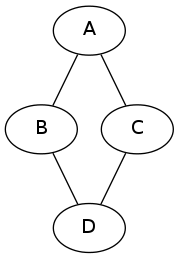
\includegraphics[width=100px]{Ia.png}
\end{figure}

\section{d-Séparation}

\subsection{Question a}


\subsection{Question b}

\subsection{Question c}

\begin{itemize}
\item L'assertion $X_{\{1, 2\}} \upmodels X_4 \mid X_3$ est fausse: ${1, 8, 4}$ n'est pas
bloqué par $4$.
\item L'assertion $X_{\{1, 2\}} \upmodels X_4 \mid X_5$ est fausse: le chemin précédant
n'est pas bloqué par $5$.
\item L'assertion $X_1 \upmodels X_6 \mid X_{\{2, 4, 7\}}$ est vraie. Tous les chemins
de $1$ vers $6$ sont bloqués par $7$.
\end{itemize}


\end{document}
